\documentclass[10pt,leqno]{article}

\usepackage[%
  tmargin=1.2in,bmargin=1.2in,%
  lmargin=1.8in,rmargin=1.8in,%
]{geometry}
\usepackage{fancyhdr}
\usepackage{titlesec}
\usepackage{appendix}
\usepackage{microtype}
\usepackage[hyphens]{url}
\usepackage{enumitem}
\usepackage{xspace}
\usepackage{etoolbox}
\usepackage{ifthen}
\usepackage{tikz}
\usepackage{tikz-cd}

\usepackage{amsmath}
\definecolor{darkred}{rgb}{0.5,0.0,0.0}
\usepackage[%
  colorlinks,%
  linkcolor=darkred,%
  citecolor=darkred,%
  urlcolor=darkred,%
]{hyperref}
\usepackage{amsthm,amssymb}
% \usepackage[lining,semibold]{libertine}
% \usepackage{textcomp,stmaryrd}
% \usepackage[libertine,cmintegrals,bigdelims]{newtxmath}
% \useosf
% \usepackage[%
%   cal=boondox, calscaled=0.97,%
%   bb=boondox, bbscaled=0.98,%
% ]{mathalfa}
\usepackage{cleveref}

\frenchspacing
\urlstyle{rm}

\AtBeginDocument{%
  \setlength{\abovedisplayskip}{1.5ex plus 0.3ex minus 0.3ex}%
  \setlength{\abovedisplayshortskip}{1.0ex plus 0.3ex minus 0.3ex}%
  \setlength{\belowdisplayskip}{1.5ex plus 0.3ex minus 0.3ex}%
  \setlength{\belowdisplayshortskip}{1.0ex plus 0.3ex minus 0.3ex}%
}

\let\theoldbibliography\thebibliography
\renewcommand{\thebibliography}[1]{%
  \theoldbibliography{#1}%
  \setlength{\parskip}{0ex}
  \setlength{\itemsep}{0.5ex plus 0.2ex minus 0.2ex}
  \small
}

\pagestyle{fancy}
\renewcommand{\headrulewidth}{0pt}
\renewcommand{\footrulewidth}{0pt}
\fancyhf{}
\fancyfoot[C]{\small\thepage}

\renewcommand{\title}[1]{\newcommand{\thetitle}{#1}}
\renewcommand{\author}[1]{\newcommand{\theauthor}{#1}}
\renewcommand{\date}[1]{\newcommand{\thedate}{#1}}

\renewcommand{\maketitle}{%
  \begin{center}
    {\bfseries\MakeUppercase{%
      \thetitle}}\\[2.5ex]
    {\footnotesize\MakeUppercase{%
      \theauthor}}\\[2.5ex]
    \ifthenelse{\equal{\thedate}{}}{}{%
      \small%
      \setlength{\tabcolsep}{0.2em}%
      \begin{tabular}{rl}
        original: & \thedate \\
        updated: & \today
      \end{tabular}
    }
  \end{center}
  \vspace{2.5ex}
  \thispagestyle{fancy}
}

%%%%%%%%%%%%%%%%%%%%%%%%%%%%%%%%%%%%%%%%%%%%%%%%%%%%%%%%%%%%%%%%%%%%%%

\cspreto{section}{\setcounter{equation}{0}}

\titleformat{\section}{\centering\scshape}{\thesection.}{0.4em}{}
\titlespacing{\section}{0pt}{*4}{*1}
\titleformat{\subsection}{\scshape}{\thesubsection.}{0.4em}{}
\titlespacing{\subsection}{0pt}{*2.5}{*1}

% Display format for equations
\newcommand{\crefeqfmt}[1]{
  \crefformat{#1}{(##2##1##3)}
  \Crefformat{#1}{(##2##1##3)}
  \crefrangeformat{#1}{(##3##1##4--##5##2##6)}
  \Crefrangeformat{#1}{(##3##1##4--##5##2##6)}
  \crefmultiformat{#1}{(##2##1##3}{, ##2##1##3)}{, ##2##1##3}{, ##2##1##3)}
  \Crefmultiformat{#1}{(##2##1##3}{, ##2##1##3)}{, ##2##1##3}{, ##2##1##3)}
  \crefrangemultiformat{#1}{(##3##1##4--##5##2##6}{, ##3##1##4--##5##2##6)}{, ##3##1##4--##5##2##6}{, ##3##1##4--##5##2##6)}
  \Crefrangemultiformat{#1}{(##3##1##4--##5##2##6}{, ##3##1##4--##5##2##6)}{, ##3##1##4--##5##2##6}{, ##3##1##4--##5##2##6)}
}
% Display format for sections
\newcommand{\crefsecfmt}[1]{%
  \crefformat{#1}{\S##2##1##3}
  \Crefformat{#1}{\S##2##1##3}
  \crefrangeformat{#1}{\S\S##3##1##4--##5##2##6}
  \Crefrangeformat{#1}{\S\S##3##1##4--##5##2##6}
  \crefmultiformat{#1}{\S\S##2##1##3}{ and~##2##1##3}{, ##2##1##3}{ and~##2##1##3}
  \Crefmultiformat{#1}{\S\S##2##1##3}{ and~##2##1##3}{, ##2##1##3}{ and~##2##1##3}
  \crefrangemultiformat{#1}{\S\S##3##1##4--##5##2##6}{ and~##3##1##4--##5##2##6}{, ##3##1##4--##5##2##6}{ and~##3##1##4--##5##2##6}
  \Crefrangemultiformat{#1}{\S\S##3##1##4--##5##2##6}{ and~##3##1##4--##5##2##6}{, ##3##1##4--##5##2##6}{ and~##3##1##4--##5##2##6}
}
\crefeqfmt{equation}
\crefeqfmt{enumi}
\crefeqfmt{enumii}
\crefsecfmt{section}
\crefsecfmt{subsection}
\crefsecfmt{appendix}
\crefname{part}{Part}{Parts}
\crefname{chapter}{Chapter}{Chapters}
\crefname{figure}{Figure}{Figures}

\makeatletter

\newcommand{\thmnumfont}{\bfseries}
\newcommand{\thmheadfont}{\bfseries}
\newcommand{\thmnotefont}{\bfseries}
\newcommand{\thmhorizspace}{0.4em}

\def\swappedhead#1#2#3{%
  \thmnumber{\@upn{{\thmnumfont#2}}\@ifnotempty{#1}{.\hspace{0.25em}}}%
  \thmheadfont\thmname{#1}%
  \@ifnotempty{#3}{\ \thmnote{\thmnotefont(#3)}}%
}
\swapnumbers

\newtheoremstyle{block}%
  {2.0ex plus 0.2ex minus 0.1ex}% Space above
  {2.0ex plus 0.2ex minus 0.1ex}% Space below
  {} % Body font
  {} % Indent amount
  {\thmheadfont} % Theorem head font
  {.} % Punctuation after theorem head
  {\thmhorizspace} % Space after theorem head
  {} % Theorem head spec (can be left empty, meaning ‘normal’)

\renewenvironment{proof}[1][Proof]{\par
  \pushQED{\qed}%
  \normalfont%
  \topsep1ex plus 0.2ex minus 0.1ex\relax%
  \labelsep \thmhorizspace\relax%
  \trivlist
  \item[\hskip\labelsep\thmheadfont
    #1\@addpunct{.}]\ignorespaces
}{%
  \popQED\endtrivlist\@endpefalse%
}

\makeatother

\theoremstyle{block}

\newcommand{\defthm}[2]{%
  \newtheorem{#1}[equation]{#2}%
  \crefeqfmt{#1}%
  \newtheorem*{#1*}{#2}%
}

\defthm{algorithm}{Algorithm}
\defthm{conjecture}{Conjecture}
\defthm{construction}{Construction}
\defthm{convention}{Convention}
\defthm{corollary}{Corollary}
\defthm{definition}{Definition}
\defthm{definitions}{Definitions}
\defthm{example}{Example}
\defthm{examples}{Examples}
\defthm{exercise}{Exercise}
\defthm{fact}{Fact}
\defthm{intuition}{Intuition}
\defthm{lemma}{Lemma}
\defthm{notation}{Notation}
\defthm{nothing}{}
\defthm{proposition}{Proposition}
\defthm{question}{Question}
\defthm{remark}{Remark}
\defthm{remarks}{Remarks}
\defthm{situtation}{Situation}
\defthm{theorem}{Theorem}

\setlist{%
  leftmargin=2.5em, parsep=0ex, listparindent=\parindent,
  itemsep=1.0ex, topsep=1.0ex,%
}

\setlist[enumerate, 1]{%
  label=(\alph*),%
  ref=\alph*,%
  widest=d,%
}
\setlist[enumerate, 2]{%
  label=(\roman*),%
  ref=\theenumi.\roman*,%
}
\setlist[itemize, 1]{%
  label=$\vcenter{\hbox{\footnotesize$\bullet$}}$,%
}
\setlist[itemize, 2]{label=--}

%%%%%%%%%%%%%%%%%%%%%%%%%%%%%%%%%%%%%%%%%%%%%%%%%%%%%%%%%%%%%%%%%%%%%%

\makeatletter

\let\ea\expandafter

\newcount\foreachcount

\def\foreachletter#1#2#3{\foreachcount=#1
  \ea\loop\ea\ea\ea#3\@alph\foreachcount
  \advance\foreachcount by 1
  \ifnum\foreachcount<#2\repeat}

\def\foreachLetter#1#2#3{\foreachcount=#1
  \ea\loop\ea\ea\ea#3\@Alph\foreachcount
  \advance\foreachcount by 1
  \ifnum\foreachcount<#2\repeat}

% Roman: \rA is \mathrm{A}
\def\definerm#1{%
  \ea\gdef\csname r#1\endcsname{\ensuremath{\mathrm{#1}}\xspace}}
\foreachLetter{1}{27}{\definerm}
\foreachletter{1}{27}{\definerm}
% Script: \sA is \mathscr{A}
\def\definescr#1{%
  \ea\gdef\csname s#1\endcsname{\ensuremath{\mathscr{#1}}\xspace}}
\foreachLetter{1}{27}{\definescr}
% Calligraphic: \cA is \mathcal{A}
\def\definecal#1{%
  \ea\gdef\csname c#1\endcsname{\ensuremath{\mathcal{#1}}\xspace}}
\foreachLetter{1}{27}{\definecal}
% Bold: \bA is \mathbf{A}
\def\definebold#1{%
  \ea\gdef\csname b#1\endcsname{\ensuremath{\mathbf{#1}}\xspace}}
\foreachLetter{1}{27}{\definebold}
% Blackboard Bold: \lA is \mathbb{A}
\def\definebb#1{%
  \ea\gdef\csname l#1\endcsname{\ensuremath{\mathbb{#1}}\xspace}}
\foreachLetter{1}{27}{\definebb}
% Fraktur: \ka is \mathfrak{a}, \kA is \mathfrak{A}
\def\definefrak#1{%
  \ea\gdef\csname k#1\endcsname{\ensuremath{\mathfrak{#1}}\xspace}}
\foreachletter{1}{27}{\definefrak}
\foreachLetter{1}{27}{\definefrak}
% Sans serif: \iA \is \mathsf{A}
\def\definesf#1{%
  \ea\gdef\csname i#1\endcsname{\ensuremath{\mathsf{#1}}\xspace}}
\foreachletter{1}{6}{\definesf}
\foreachletter{7}{14}{\definesf}
\foreachletter{15}{27}{\definesf}
\foreachLetter{1}{27}{\definesf}
% Bar: \Abar is \overline{A}, \abar is \overline{a}
\def\definebar#1{%
  \ea\gdef\csname #1bar\endcsname{\ensuremath{\overline{#1}}\xspace}}
\foreachLetter{1}{27}{\definebar}
\foreachletter{1}{8}{\definebar} % \hbar is something else!
\foreachletter{9}{15}{\definebar} % \obar is something else!
\foreachletter{16}{27}{\definebar}
% Tilde: \Atil is \widetilde{A}, \atil is \widetilde{a}
\def\definetil#1{%
  \ea\gdef\csname #1til\endcsname{\ensuremath{\widetilde{#1}}\xspace}}
\foreachLetter{1}{27}{\definetil}
\foreachletter{1}{27}{\definetil}
% Hats: \Ahat is \widehat{A}, \ahat is \widehat{a}
\def\definehat#1{%
  \ea\gdef\csname #1hat\endcsname{\ensuremath{\widehat{#1}}\xspace}}
\foreachLetter{1}{27}{\definehat}
\foreachletter{1}{27}{\definehat}
% Checks: \Achk is \widecheck{A}, \achk is \widecheck{a}
\def\definechk#1{%
  \ea\gdef\csname #1chk\endcsname{\ensuremath{\widecheck{#1}}\xspace}}
\foreachLetter{1}{27}{\definechk}
\foreachletter{1}{27}{\definechk}
% Underline: \Aund is \underline{A}, \aund is \underline{a}
\def\defineul#1{%
  \ea\gdef\csname #1und\endcsname{\ensuremath{\underline{#1}}\xspace}}
\foreachLetter{1}{27}{\defineul}
\foreachletter{1}{27}{\defineul}

\makeatother

%%%%%%%%%%%%%%%%%%%%%%%%%%%%%%%%%%%%%%%%%%%%%%%%%%%%%%%%%%%%%%%%%%%%%%

\usetikzlibrary{calc,decorations.pathmorphing,shapes,arrows}
\tikzcdset{
  arrow style=tikz,
  diagrams={>={stealth}},
}

\newcommand{\arrlen}{1em}
\renewcommand{\to}{\mathrel{\tikz[baseline]%
    \draw[>=stealth,->](0,0.5ex)--(\arrlen,0.5ex);}}
\newcommand{\from}{\mathrel{\tikz[baseline]%
    \draw[>=stealth,<-](0,0.5ex)--(\arrlen,0.5ex);}}
\renewcommand{\mapsto}{\mathrel{\tikz[baseline]%
    \draw[>=stealth,|->](0,0.5ex)--(\arrlen,0.5ex);}}
\newcommand{\inj}{\mathrel{\tikz[baseline]%
    \draw[>=stealth,right hook->](0,0.5ex)--(\arrlen,0.5ex);}}
\newcommand{\surj}{\mathrel{\tikz[baseline]%
    \draw[>=stealth,->>](0,0.5ex)--(\arrlen,0.5ex);}}
\newcommand{\fromto}{\mathrel{%
  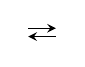
\begin{tikzpicture}[baseline]%
    \draw[>=stealth,<-](0,0.15ex)--(\arrlen,0.15ex);%
    \draw[>=stealth,->](0,0.85ex)--(\arrlen,0.85ex);%
  \end{tikzpicture}}}
\newcommand{\doubto}{\mathrel{%
  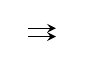
\begin{tikzpicture}[baseline]%
    \draw[>=stealth,->](0,0.15ex)--(\arrlen,0.15ex);%
    \draw[>=stealth,->](0,0.85ex)--(\arrlen,0.85ex);%
  \end{tikzpicture}}}
\newcommand{\lblto}[1]{\mathrel{%
    \begin{tikzpicture}[baseline= {( $ (current bounding box.south) + (0,-0.5ex) $ )}]
      \node[inner sep=.4ex] (a) {\,$\scriptstyle #1$\,};
      \draw[>=stealth,->] (a.south west) -- (a.south east);
    \end{tikzpicture}}}
\newcommand{\isoto}{\lblto{\sim}}

\newcommand{\simpl}[3]{
  \begin{tikzcd}[ampersand replacement=\&, column sep=small]
    #1 \&
    #2 \ar[l, shift right=0.35ex]
       \ar[l, shift left=0.35ex] \&
    #3 \ar[l, shift right=0.70ex]
       \ar[l, shift left=0.70ex]
       \ar[l] \&
    \cdots \ar[l, shift right=0.35ex]
           \ar[l, shift left=0.35ex]
           \ar[l, shift right=1.05ex]
           \ar[l, shift left=1.05ex]
  \end{tikzcd}
}
\newcommand{\cosimpl}[3]{
  \begin{tikzcd}[ampersand replacement=\&, column sep=small]
    #1 \ar[r, shift right=0.35ex]
       \ar[r, shift left=0.35ex] \&
    #2 \ar[r, shift right=0.70ex]
       \ar[r, shift left=0.70ex]
       \ar[r] \&
    #3 \ar[r, shift right=0.35ex]
       \ar[r, shift left=0.35ex]
       \ar[r, shift right=1.05ex]
       \ar[r, shift left=1.05ex] \&
    \cdots
  \end{tikzcd}
}

\newcommand{\tto}{\mathrel{\tikz[baseline]%
    \draw[>=stealth,->,double, double distance = 0.3ex](0,0.5ex)--(\arrlen,0.5ex);}}
\newcommand{\doubfrom}{\mathrel{%
  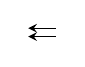
\begin{tikzpicture}[baseline]%
    \draw[>=stealth,<-](0,0.15ex)--(\arrlen,0.15ex);%
    \draw[>=stealth,<-](0,0.85ex)--(\arrlen,0.85ex);%
  \end{tikzpicture}}}
\newcommand{\tripfrom}{\mathrel{%
  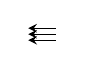
\begin{tikzpicture}[baseline]%
    \draw[>=stealth,<-](0,0.00ex)--(\arrlen,0.00ex);%
    \draw[>=stealth,<-](0,0.50ex)--(\arrlen,0.50ex);%
    \draw[>=stealth,<-](0,1.00ex)--(\arrlen,1.00ex);%
  \end{tikzpicture}}}


\renewcommand{\l}{\left}
\renewcommand{\r}{\right}
\newcommand{\f}{\frac}
\renewcommand{\o}{\overline}
\renewcommand{\u}{\underline}
\newcommand{\til}{\widetilde}
\renewcommand{\hat}{\widehat}
\newcommand{\del}{\partial}
\newcommand{\dash}{\text{-}}
\renewcommand{\c}{\colon}
\newcommand{\lc}{\,:\!}
\newcommand{\ce}{\coloneq}%{\mathrel{:=}}
\newcommand{\ec}{\eqcolon}%{\mathrel{=:}}
\newcommand{\iso}{\simeq}
\newcommand{\dual}{\vee}
\newcommand{\ldb}{\llbracket}
\newcommand{\rdb}{\rrbracket}

\newcommand{\Obj}{\operatorname{Obj}}
\newcommand{\Hom}{\operatorname{Hom}}
\newcommand{\Map}{\operatorname{Map}}
\newcommand{\Fun}{\operatorname{Fun}}
\newcommand{\Aut}{\operatorname{Aut}}
\newcommand{\Iso}{\operatorname{Iso}}
\renewcommand{\id}{\mathrm{id}}
\renewcommand{\im}{\operatorname{im}}
\newcommand{\op}{\mathrm{op}}
\newcommand{\univ}{\mathrm{univ}}
\newcommand{\colim}{\operatorname*{colim}}
\newcommand{\dlim}{\displaystyle\lim}
\newcommand{\dcolim}{\displaystyle\colim}
\newcommand{\Spec}{\operatorname{Spec}}
\newcommand{\Spf}{\operatorname{Spf}}

%%%%%%%%%%%%%%%%%%%%%%%%%%%%%%%%%%%%%%%%%%%%%%%%%%%%%%%%%%%%%%%%%%%%%%


\title{$D$-modules, representation theory, Hodge theory}
\author{Arpon Raksit}
\date{March 15, 2016}

%%%%%%%%%%%%%%%%%%%%%%%%%%%%%%%%%%%%%%%%%%%%%%%%%%%%%%%%%%%%%%%%%%%%%%

\newcommand{\an}{\mathrm{an}}
\newcommand{\dR}{\mathrm{dR}}
\newcommand{\Gr}{\operatorname{Gr}}
\newcommand{\hol}{\mathrm{hol}}
\newcommand{\QCoh}{\mathrm{QCoh}}
\newcommand{\Sch}{\mathrm{Sch}}
\newcommand{\sing}{\mathrm{sing}}
\newcommand{\sm}{\mathrm{sm}}

%%%%%%%%%%%%%%%%%%%%%%%%%%%%%%%%%%%%%%%%%%%%%%%%%%%%%%%%%%%%%%%%%%%%%%

\begin{document}
\maketitle
\thispagestyle{empty}

% \begin{abstract}
%   One perspective on classical Hodge theory is that it is the study of the information contained in the complex cohomology of complex varieties. Complex cohomology is perhaps usually thought of as an invariant of the complex-analytic space underlying a variety, but it may be constructed purely algebraically, via algebraic de Rham cohomology. In this essay we discuss aspects of Hodge theory that are visible from this purely algebraic point of view, namely the degeneration of the Hodge--de Rham spectral sequence (by an argument of Deligne-Illusie) and the Gauss-Manin connection (which we also examine from the perspective of crystals).
% \end{abstract}

% \tableofcontents
% \newpage

% \section*{Acknowledgements}

\begin{itemize}[leftmargin=*]
\item Thanks to Prof. Ian Grojnowski for suggesting this essay topic and for supervising my reading.
\item I am very grateful to Harvard University and the Herchel Smith Fellowship for generously supporting me and giving me the opportunity to come to Cambridge this year.
\end{itemize}

\newpage

\numberwithin{block}{subsection}
\cspreto{section}{\setcounter{block}{0}}
\addtocounter{section}{-1}

\section{Introduction}
\label{intro}

Let's say we're interested in studying algebraic varieties $X$ over a field $K$. In the classical case where $K = \lC$, we are abetted by the fact that, in addition to the Zariski topology on $X$, we have a natural analytic topology on the set of complex points $X(\lC)$. More precisely, the set $X(\lC)$ carries the structure of a complex-analytic space (a complex manifold when $X$ is smooth), referred to as the \emph{analytification} of $X$ and denoted $X^\an$. While the Zariski topology is certainly very useful, the analytic topology is much closer to our intuitive notion of what a complex variety looks like, so we might seek to gain information about $X$ by studying $X^\an$ topologically.

There's a natural tool we might employ in approaching the latter task: complex cohomology. There are several perspectives on this tool, but let us take as our starting point the sheaf-theoretic formulation.

\begin{definition}
  \label{intro--complex-cohom}
  We define the \emph{complex cohomology} of a topological space $U$ as the sheaf cohomology $\rH^*(U;\u\lC)$, where $\u\lC$ denotes the constant sheaf on $U$ with value $\lC$.
\end{definition}

So we are looking at $\rH^*(X^\an,\u\lC)$ as an invariant of $X^\an$, and hence of $X$. To justify our statement above abut the advantage of the analytic topology, let us note that this is completely different from considering $\rH^*(X;\u\lC)$, the complex cohomology of $X$ equipped with its Zariski topology, which is of much less interest. Indeed, if $X$ is an irreducible variety, then the constant sheaf $\u\lC$ on it is flasque, hence acyclic. For example, suppose $X$ is complex projective space $\lP^n_\lC$; then $X$ is irreducible as a variety, so $\rH^r(X;\u\lC) \iso 0$ for $r > 0$, while $X^\an$, complex projective space as a complex manifold, has nontrivial complex cohomology.

But what if we are interested in working over some other field $K$? Is there some way we can still employ such cohomological invariants? We are brought to the following motivating question.

\begin{question}
  \label{intro--q-alg}
  Can the invariant $\rH^*(X^\an;\u\lC)$ of $X$ be constructed and studied purely algebraically (i.e. intrinsically to $X$, without resorting to the analytic object\footnote{The diction here is ironic: this essay is written by an author and aimed at a reader who would only under significant duress resort in the lands of analysis. It is left to the reader to decide whether this is a warning against or an encouragement towards continuing.} $X^\an$)?
\end{question}

There's another concern we might have even when working over $\lC$. A priori, the invariant $\rH^*(X^\an;\lC)$ is sensitive only to the homotopy type of $X^\an$. This is somewhat unsatisfactory from the point of view of geometry. For example, for any elliptic curve $X$, $X^\an$ is homeomorphic to a torus. Thus, a priori, complex cohomology cannot distinguish between non-isomorphic elliptic curves. This motivates a second question.

\begin{question}
  \label{intro--q-struct}
  Is there extra structure carried by $\rH^*(X^\an;\u\lC)$ that is sensitive to the holomorphic structure of $X^\an$ and the algebraic structure of $X$?
\end{question}

The above two questions can be addressed using the de Rham perspective on cohomology, which is the main subject of this essay.

%%%%%%%%%%%%%%%%%%%%%%%%%%%%%%%%%%%%%%%%%%%%%%%%%%%%%%%%%%%%%%%%%%%%%%

\subsection{Hodge theory}
\label{intro--hodge}

Let us first addess \cref{intro--q-struct}. We begin by recalling how to bridge the sheaf-theoretic definition of complex cohomology above with the de Rham perspective. This centers around ``resolving'' the sheaf $\u\lC$ by sheaves of differential forms. However, there are variations on this theme, resulting in different formulations of de Rham cohomology. It is instructive to begin by considering the usual formulation from differential topology, even though it won't be of further interest to us here.

\begin{situation}
  \label{intro--hodge--hyp}
  In this subsection, let $\sX$ be a complex manifold of complex dimension $n$ (so of dimension $2n$ as a smooth manifold), perhaps imagining $\sX = X^\an$ for $X$ a smooth variety of dimension $n$ over $\lC$.
\end{situation}

\begin{definition}
  \label{intro--hodge--smooth-derham}
  Let $\Omega_{\sX,\sm}^\bullet$ denote the cochain-complex of sheaves of smooth complex differential forms on $\sX$. Define the (complex) \emph{smooth de Rham cohomology} of $\sX$ as
  \[
    \rH^*_{\dR,\sm}(\sX) \ce
    \rH^*(\sX;\Omega_{\sX,\sm}^\bullet),
  \]
  the sheaf cohomology\footnote{When evaluated on cochain-complexes of sheaves, sheaf cohomology is sometimes referred to as \emph{hypercohomology}. I don't care for this terminology.} of this cochain-complex.
\end{definition}

This definition may initially come across as opaque or abstruse, but it is the one that we will be able to immediately emulate in the variations that follow. In any case, let us quickly show that it computes complex cohomology and is equivalent to the more standard definition.

\begin{nothing}
  \label{intro--hodge--smooth-derham-iso}
  The classical Poincar\'e lemma for smooth forms implies that the sequence of sheaves
  \[
    0 \to \u\lC \to \Omega^0_{\sX,\sm} \lblto{d}
    \Omega^1_{\sX,\sm} \lblto{d} \cdots \lblto{d}
    \Omega^{2n}_{\sX,\sm} \to 0
  \]
  is exact. In other words, viewing the sheaf $\u\lC$ as a cochain-complex concentrated in degree $0$, we have a canonical quasi-isomorphism
  $\u\lC \isoto \Omega_{\sX,\sm}^\bullet$, begetting a canonical isomorphism
  \[
    \rH^*(\sX,\u\lC) \isoto \rH^*_{\dR,\sm}(\sX)
  \]
  between complex cohomology and smooth de Rham cohomology.
\end{nothing}

\begin{nothing}
  \label{intro--hodge--smooth-derham-global}
  The sheaves $\Omega_{\sX,\sm}^i$ are acyclic---i.e. $\rH^j(\sX;\Omega_{\sX,\sm}^i) \iso 0$ for $j > 0$---due to the existence of smooth partitions of unity. Hence the sheaf cohomology of $\Omega_{\sX,\sm}^\bullet$ may be computed as the cohomology of its cochain-complex of global sections, i.e.
  \[
    \rH^*_{\dR,\sm}(\sX) \iso
    \rH^*(\Gamma(\sX,\Omega_{\sX,\sm}^\bullet)).
  \]
\end{nothing}

While this familiar characterization of smooth de Rham cohomology provides a concrete way of understanding cohomology classes, it's not of great help in formulating cohomology algebraically. However, it does give us a template that we can translate into both the holomorphic and algebraic settings, which by GAGA principles we should be able to compare. So let's do that. We first address the holomorphic case.

\begin{definition}
  \label{intro--hodge--holomorphic-derham}
  Let $\Omega_{\sX}^\bullet$ denote the cochain-complex of sheaves of holomorphic complex differential forms on $\sX$ and define the \emph{holomorphic de Rham cohomology} of $\sX$ as
  \[
    \rH^*_\dR(\sX) \ce
    \rH^*(\sX;\Omega_{\sX}^\bullet),
  \]
  the sheaf cohomology of this cochain-complex.
\end{definition}

\begin{nothing}
  \label{intro--hodge--holomorphic-derham-iso}
  There is a holomorphic analogue of the Poincar\'e lemma, implying that the sequence of sheaves
  \[
    0 \to \u\lC \to \Omega^0_{\sX} \lblto{\del}
    \Omega^1_{\sX} \lblto{\del} \cdots \lblto{\del}
    \Omega^n_{\sX} \to 0
  \]
  is exact. Again, this may be reformulated as a quasi-isomorphism $\u\lC \isoto \Omega_{\sX}^\bullet$, begetting a canonical isomorphism
  \[
    \rH^*(\sX,\u\lC) \isoto \rH^*_\dR(\sX)
  \]
  between complex cohomology and holomorphic de Rham cohomology.
\end{nothing}

\begin{nothing}
  \label{intro--hodge--holomorphic-derham-nonglobal}
  Unlike the smooth situation \cref{intro--hodge--smooth-derham-global}, the holomorphic sheaves $\Omega^i_{\sX}$ are not in general acyclic (we do not have holomorphic partitions of unity). Thus, holomorphic de Rham cohomology cannot in general be identified as the cohomology of the cochain-complex of global holomorphic differential forms.
\end{nothing}

\begin{nothing}
  \label{intro--hodge--holomorphic-hodge-ss}
  However, there is still a sense in which holomorphic de Rham cohomology is controlled by the individual sheaves $\Omega^i_{\sX}$. Namely, there is a spectral sequence
  \[
    E^{i,j}_1 = \rH^j(\sX;\Omega^i_{\sX})
    \quad \Rightarrow \quad
    \rH^{i+j}_\dR(\sX),
  \]
  which we refer to as the \emph{Hodge--de Rham spectral sequence}.

  This spectral sequence arises from a filtration on the complex of sheaves $\Omega_{\sX}^\bullet$, namely the ``stupid filtration''
  \[
    0 = \Omega_{\sX}^{\bullet \ge n+1}
    \inj \cdots \inj \Omega_{\sX}^{\bullet \ge i} \inj \cdots \inj
    \Omega_{\sX}^{\bullet \ge 0} = \Omega_{\sX}^\bullet,
  \]
  where $\Omega_{\sX}^{\bullet \ge i}$ is the truncation of $\Omega_{\sX}^\bullet$ to a cochain-complex concentrated in degrees $\ge i$. In particular, the spectral sequence converges to the (associated graded of the) filtration
  \[
    0 = F^{n+1}\rH_\dR^r(\sX)
    \inj \cdots \inj F^i\rH_\dR^r(\sX) \inj \cdots \inj
    F^0\rH_\dR^r(\sX) = \rH_\dR^r(\sX),
  \]
  where $F^i\rH_\dR^r(\sX)$ is the image of the map on sheaf cohomology induced by the inclusion $\Omega_{\sX}^{\bullet \ge i} \inj \Omega_{\sX}^\bullet$; we call this filtration on holomorphic de Rham cohomology the \emph{Hodge filtration}.
\end{nothing}

This is the beginning of our answer to \cref{intro--q-struct}: the complex cohomology of $\sX$ carries the extra structure of this Hodge filtration. Seeking to better understand this structure, we are naturally brought to the following question.

\begin{question}
  \label{intro--hodge--q-degen}
  What can we say about the degeneration of the holomorphic Hodge--de Rham spectral sequences \cref{intro--hodge--holomorphic-hodge-ss}?
\end{question}

This question is answered by the main theorem of Hodge theory, which can be formulated as follows.

\begin{nothing}
  \label{intro--hodge--conjugation}
  By functoriality of sheaf cohomology, the complex conjugation automorphism on $\u\lC$ determines a complex conjugation automorphism on complex cohomology $\rH^*(\sX,\u\lC)$, and hence on holomorphic de Rham cohomology $\rH_\dR^*(\sX)$ via the isomorphism \cref{intro--hodge--holomorphic-derham-iso}. One may alternatively think of this conjugation operation as the ``real structure'' arising from  the canonical isomorphism
  \[
    \rH^*(\sX,\u\lR) \otimes_\lR \lC \isoto \rH^*(\sX,\u\lC).
  \]
\end{nothing}

\begin{notation}
  \label{intro--hodge--conjugate-filtration}
  We denote by $\o F$ the filtration on $\rH_\dR^*(\sX)$ conjugate to the Hodge filtration $F$ under the conjugation automorphism defined in \cref{intro--hodge--conjugation}.
\end{notation}
 
\begin{theorem}
  \label{intro--hodge--theory}
  Suppose $\sX$ is compact and K\"ahler (which holds e.g. when $\sX = X^\an$ for $X$ a smooth \emph{projective} complex variety).
  \begin{enumerate}[leftmargin=*]
  \item \label{intro--hodge--theory--degen}
    The holomorphic Hodge--de Rham spectral sequence \cref{intro--hodge--holomorphic-hodge-ss} degenerates immediately at $E_1$. We thus have canonical isomorphisms
    \[
      \Gr_F^p\rH_\dR^{p+q}(\sX) \iso \rH^q(\sX;\Omega^p_{\sX}),
    \]
    where $\Gr_F^\bullet$ is the associated graded of the Hodge filtration.
  \item \label{intro--hodge--theory--split}
    The composite map
    \[
      F^i\rH_\dR^{i+j}(\sX) \cap \o F^j\rH_\dR^{i+j}(\sX) \inj F^i\rH_\dR^{i+j}(\sX) \surj \Gr_F^i\rH_\dR^{i+j}(\sX)
    \]
    is an isomorphism. We thus have a canonical splitting
    \[
      \rH_\dR^k(\sX) \iso \bigoplus_{0 \le i \le k} \Gr_F^i\rH_\dR^k(\sX) \iso \bigoplus_{i+j=k} \rH^j(\sX;\Omega^i_{\sX}),
    \]
    in which the subspaces $\rH^j(\sX;\Omega^i_{\sX})$ and $\rH^i(\sX;\Omega^j_{\sX})$ are conjugates of one another.
  \end{enumerate}
\end{theorem}

\begin{remark}
  \label{intro--hodge--constraint}
  Note that in addition to allowing us to understand the Hodge filtration, \cref{intro--hodge--theory} immediately places some concrete cohomological restrictions on compact K\"ahler manifolds $\sX$. For example, we see that $\rH^j(\sX;\Omega^i_{\sX})$ and $\rH^i(\sX;\Omega^j_{\sX})$ must have the same dimension (as $\lC$-vector spaces), and hence that $\rH^k(\sX;\u\lC) \iso \rH_\dR^k(\sX)$ must have even dimension when $k$ is odd.
\end{remark}

%%%%%%%%%%%%%%%%%%%%%%%%%%%%%%%%%%%%%%%%%%%%%%%%%%%%%%%%%%%%%%%%%%%%%%

\subsection{Algebraic de Rham cohomology}
\label{intro--alg}

We now address \cref{intro--q-alg}, by formulating an algebraic analogue of de Rham cohomology.

\begin{situation}
  \label{intro--alg--hyp}
  In this subsection we let $K$ be any field and $X$ a $K$-scheme.
\end{situation}

\begin{notation}
  \label{intro--kahler-differentials}
  Let $\Omega_{X/K}$ denote the sheaf of relative K\"ahler differentials for the structure morphism $X \to \Spec K$. Recall that this object plays the role of the cotangent bundle in the algebraic world, in particular coming equipped with a canonical ``differential'' map $d \c \sO_X \to \Omega_{X/K}$.
\end{notation}

\begin{definition}
  \label{intro--algebraic-derham}
   Let $\Omega_{X/K}^i$ be the $i$-th exterior power of $\Omega_{X/K}$ (as an $\sO_X$-module) for $i\ge 0$. The differential $d \c \sO_X \to \Omega_{X,K}$ induces differentials $\Omega_{X/K}^i \to \Omega_{X/K}^{i+1}$, giving rise to a cochain-complex of sheaves $\Omega_{X/K}^\bullet$ called the \emph{de Rham complex} of $X$ over $K$. We think of this as the cochain-complex of ``algebraic differential forms'' on $X$ and define the \emph{algebraic de Rham cohomology} of $X$ as
  \[
    \rH^*_\dR(X) \ce \rH^*(X;\Omega_{X/K}^\bullet),
  \]
  the sheaf cohomology of this cochain-complex.
\end{definition}

\begin{nothing}
  \label{intro--alg--hodge-ss}
  The construction of the Hodge--de Rham spectral sequence in the holomorphic setting \cref{intro--hodge--holomorphic-hodge-ss} goes through verbatim for algebraic de Rham cohomology, giving an algebraic \emph{Hodge--de Rham spectral sequence}
  \[
    E^{i,j}_1 = \rH^j(\sX;\Omega^i_{\sX})
    \quad \Rightarrow \quad
    \rH^{i+j}_\dR(\sX)
  \]
  convering to an algebraic \emph{Hodge filtration}.
\end{nothing}

Now, in the case $K = \lC$, Serre's GAGA allows us to compare algebraic and holomorphic de Rham cohomology, giving the following.

\begin{theorem}
  \label{intro--alg--gaga}
  Suppose $K = \lC$ and $X$ is proper. There are natural isomorphisms
  \[
    \rH^j(X;\Omega_{X/\lC}^i) \iso \rH^j(X^\an;\Omega_{X^\an}^i).
  \]
  These extend to a natural isomorphism between the holomorphic and algebraic Hodge--de Rham spectral sequences \cref{intro--hodge--holomorphic-hodge-ss,intro--alg--hodge-ss}. Consequently, there is a natural isomorphism
  \[
    \rH_\dR^*(X) \iso \rH_\dR^*(X^\an)
  \]
  between the algebraic de Rham cohomology of $X$ and the holomorphic de Rham cohomology of $X^\an$, under which the holomorphic and algebraic Hodge filtrations may be identified.
\end{theorem}

Together with \cref{intro--hodge--holomorphic-derham-iso}, this provides the beginning of an answer to \cref{intro--q-alg}: for $K = \lC$, the algebraic de Rham cohomology of $X$ is a purely algebraic construction of the complex cohomology of $X^\an$. But we might further wonder whether or not we may make purely algebraic arguments in studying de Rham cohomology.

For instance, note that our GAGA result \cref{intro--alg--gaga} also shows that the degeneration of the holomorphic Hodge--de Rham spectral sequence \cref{intro--hodge--theory--degen} immediately implies the same result for the algebraic analogue:

\begin{corollary}
  \label{intro--alg--degen}
  Suppose $K = \lC$ and $X$ is proper. The algebraic Hodge--de Rham spectral sequence \cref{intro--alg--hodge-ss} degenerates immediately at $E_1$.
\end{corollary}

We stated this result in its holomorphic guise first because classically Hodge theory is an analytic theory; in particular, the proof of \cref{intro--hodge--theory} relies heavily on analytic methods. But we've now ended up with this purely algebraic consequence, and it is natural to wonder whether it has a purely algebraic proof. More generally, we may wonder which aspects of Hodge theory or what structures on de Rham cohomology are visible from the purely algebraic perspective. These wonderings are precisely what will concern us in this essay.
%%%%%%%%%%%%%%%%%%%%%%%%%%%%%%%%%%%%%%%%%%%%%%%%%%%%%%%%%%%%%%%%%%%%%%

\subsection{Overview}

In \cref{degen} we present a purely algebraic proof due to Deligne-Illusie for the degeneration of the algebraic Hodge--de Rham spectral sequence in characteristic zero. Interestingly, the proof crucially involves studying the situation in characteristic $p$.

In \cref{gm} we study how de Rham cohomology varies in families. That is, we will consider the more general situation where we replace our variety $X \to \Spec k$ with an arbitrary map of schemes $X \to S$. In this case we will see there is further structure on de Rham cohomology related to local systems and connections.



\newpage

\section{Hodge--de Rham degeneration}
\label{degen}

The  goal of this section is to present Deligne-Illusie's algebraic argument for the following theorem.

\begin{theorem}
  \label{degen--main}
  Suppose $K$ is a field of characteristic zero and $X$ is a smooth, proper $K$-scheme. Then the Hodge--de Rham spectral sequence 
  \[
    E_1^{i,j} = \rH^j(X;\Omega_{X/K}^i)
    \quad \Rightarrow \quad
    \rH_\dR^{i+j}(X/K)
  \]
  degenerates immediately at $E_1$.
\end{theorem}

\begin{nothing}
  \label{degen--strategy}
  Let's begin with a rough intuition for the Deligne-Illusie strategy. First, note that, since $X$ is proper, the Hodge--de Rham spectral sequence is a spectral sequence of \emph{finite-dimensional} $K$-vector spaces, so we always have the inequality
  \[
    \dim_K \rH_\dR^k(X/K) \le \sum_{i+j=k} \dim_K \rH^j(X;\Omega_{X/K}^i),
  \]
  with equality holding if and only if the spectral sequence degenerates at $E_1$. In particular, to prove degeneration it would suffice to give any isomorphism
  \[
    \rH_\dR^k(X/K) \iso \bigoplus_{i+j=k} \rH^j(X;\Omega_{X/K}^i).
  \]
  The left-hand side is by definition the $k$-th sheaf cohomology group of the de Rham complex $\Omega_{X/K}^\bullet$; if we view the sheaf $\Omega_{X/K}^i$ as a cochain-complex concentrated in degree $i$, then the right-hand side may be reformulated as the $k$-th sheaf cohomology group of the cochain-complex $\bigoplus_i \Omega_{X/K}^i[-i]$, which has the same components as the de Rham complex but trivial differential. It would thus suffice to give an equivalence
  \begin{equation}
    \label{degen--strategy--desire-lift}
    \Omega_{X/K}^\bullet \iso \bigoplus_i \Omega_{X/K}^i[-i]
  \end{equation}
  in the derived category of $X$. Of course, for this to exist, the cohomology sheaves of these two complexes would need to be isomorphic, i.e. we would need
  \begin{equation}
    \label{degen--strategy--desire}
    \rH^i(\Omega_{X/K}^\bullet) \iso \Omega_{X/K}^i.
  \end{equation}

  To investigate the plausibility of this statement, let's consider a very simple example: $X \ce \lA^1_K = \Spec K[t]$. As $X$ is affine, we may think of quasi-coherent sheaves on $X$ simply as their $K[t]$-modules of global sections. The sheaf $\Omega_{X/K}^1$ is free of rank $1$, generated by $dt$, so the de Rham complex is concentrated in degrees $0$ and $1$, given simply by the differentiation map
  \[
    K[t] \lblto{d} K[t]dt.
  \]
  The key observation is that this complex behaves very differently in positive characteristic than it does in characteristic zero.
  
  If $K$ has characteristic $0$, $d$ is surjective and the kernel of $d$ is given simply by the constants $K$, so we recover the usual cohomology of affine space:
  \[
    \rH^0(\Omega_{X/K}^\bullet) = K, \quad
    \rH^1(\Omega_{X/K}^\bullet) = 0,
  \]
  so \cref{degen--strategy--desire} certainly does not hold.

  If $K$ has characteristic $p > 0$, then the fact that $t^p$ has derivative $pt^{p-1} = 0$ implies that the kernel of $d$ consists of polynomials of the form $f(t^p)$, and the cokernel of $d$ consists of $1$-forms of the form $t^{p-1}f(t)dt$. That is we have,
  \[
    \rH^0(\Omega_{X/K}^\bullet) = K[t^p] \iso K[t], \quad \rH^0(\Omega_{X/K}^\bullet) = t^{p-1}K[t]dt \iso K[t]dt,
  \]
  which suggests that, modulo the intervention of the $p$-th-powers, something like \cref{degen--strategy--desire} may indeed hold!

  The conclusion is that the strategy outlined above may yield degeneration results in positive characteristic. This is indeed the case. In \cref{degen--cartier} we will formulate the precise version of the isomorphism \cref{degen--strategy--desire} that holds in characteristic $p> 0$, taking into account the $p$-th powers. In \cref{degen--lift} we will study when this isomorphism may be lifted to an equivalence \cref{degen--strategy--desire-lift} in the derived category, and show that when such a lift exists we obtain a degeneration result. Finally, in \cref{degen--final} we will indicate how these positive characteristic results in fact imply the desired characteristic zero result.
\end{nothing}

%%%%%%%%%%%%%%%%%%%%%%%%%%%%%%%%%%%%%%%%%%%%%%%%%%%%%%%%%%%%%%%%%%%%%%

\subsection{The Cartier isomorphism}
\label{degen--cartier}

Throughout this subsection and the next we fix a prime $p$. We first discuss $p$-th power maps.

\begin{definition}
  \label{degen--cartier--frobenius}
  \begin{enumerate}[leftmargin=*]
  \item We say a scheme $X$ is of \emph{characteristic $p$} if $p\sO_X = 0$, or equivalently if the unique map $X \to \Spec \lZ$ factors through $\Spec \lF_p$.
  \item If $X$ is a scheme of characteristic $p$, then there is an \emph{ absolute Frobenius map} $F_X \c X \to X$ which is the identity map on the underlying topological space of $X$ and is given by the $p$-th power map $a \mapsto a^p$ on the structure sheaf $\sO_X$.
  \item Let $f \c X \to S$ be a map of schemes of characteristic $p$. The diagram
    \begin{equation}
      \label{degen--cartier--frobenius--commute}
      \begin{tikzcd}
        X \ar[r, "F_X"] \ar[d, "f"] &
        X \ar[d, "f"] \\
        S \ar[r, "F_S"] &
        S
      \end{tikzcd}
    \end{equation}
    evidently commutes. Define the scheme $X'$ (also denoted $X'_S$) and maps $G_{X/S} \c X' \to X$ and $f' \c X' \to S$ by the pullback diagram
    \[
      \begin{tikzcd}
        X' \ar[r, "G_{X/S}"] \ar[d, "f'"] &
        X \ar[d, "f"] \\
        S \ar[r, "F_S"] &
        S,
      \end{tikzcd} 
    \]
    and define the \emph{relative Frobenius map} $F_{X/S} \c X \to X'$ to be the map determined by \cref{degen--cartier--frobenius--commute}.
  \end{enumerate}
\end{definition}

\begin{situation}
  For the remainder of this subsection and the next, let $f \c X \to S$ be a map of schemes of characteristic $p$.
\end{situation}

\begin{lemma}
  \label{degen--cartier--frobenius-homeo}
  At the level of topogical spaces, the maps $F_{X/S}$ and $G_{X/S}$ are inverse homeomorphisms. In addition, $F_{X/S}$ is universally injective (i.e. injective after any base change).
\end{lemma}

\begin{proof}
  By definition we have $G_{X/S}F_{X/S} = F_X$, and one easily checks that $F_{X/S}G_{X/S} = F_{X'}$. Since the absolute Frobenius map is by definition the identity on topological spaces, it follows that $F_{X/S}$ and $G_{X/S}$ are homeomorphisms. Since $G_{X/S}$ is an arbitrary base change of $F_S$, this proves that an absolute Frobenius map is a universal homeomorphism. Thus $G_{X/S}F_{X/S} = F_X$ is a universal homeomorphism, proving $F_{X/S}$ is universally injective.
\end{proof}

\begin{nothing}
  \label{degen--cartier--frobenius-id}
  By \cref{degen--cartier--frobenius-homeo}, we can think of $X'$ as having the same underlying topological space as $X$. Indeed, in what follows we will make this (perhaps abusive) identification, which allows us to omit the pushforward and inverse-image functors $(F_{X/S})_*,F_{X/S}^{-1},(G_{X/S})_*,G_{X/S}^{-1}$ from our notation.

  The structure sheaf $\sO_{X'}$ is then the sheaf on $X$ given by $f^{-1}\sO_S \otimes_{f^{-1}\sO_S}\sO_X $, where the left-hand $f^{-1}\sO_s$ is viewed as a module over the base $f^{-1}\sO_S$ via the Frobenius $F_S$. So sections of $\sO_{X'}$ are locally of the form $a \otimes t$ for $a$ a section of $f^{-1}\sO_S$ and $t$ a section of $\sO_X$. In these terms:
  \begin{itemize}
  \item $G_{X/S} \c X' \to X$ is given by the map $G_{X/S}^\sharp \c \sO_X \to \sO_{X'}$ sending $at \mapsto a^p \otimes t$;
  \item $F_{X/S} \c X \to X'$ is given be the map $F_{X/S}^\sharp \c \sO_{X'} \to \sO_X$ sending $a \otimes t \mapsto at^p$.
  \end{itemize}
  This perhaps is clearest in the following example.
\end{nothing}

\begin{example}
  \label{degen--cartier--frobenius-eg}
  Let $S \ce \Spec A$ for a ring $A$ of characteristic $p$ and $X \ce \lA^n_S = \Spec A[t_1,\ldots,t_n]$, and consider the canonical map $f \c X \to S$. The scheme $X'$ is also isomorphic to $\lA^n_S$ and:
  \begin{itemize}
  \item the map $G_{X/S} \c X' \to X$ corresponds to the map $A[t_1,\ldots,t_n] \to A[t_1,\ldots,t_n]$ sending $at_i \mapsto a^pt_i$ for $a \in A$;
  \item the relative Frobenius $F_{X/S} \c X \to X'$ corresponds to the map $A[t_1,\ldots,t_n] \to A[t_1,\ldots,t_n]$ sending $at_i \mapsto at_i^p$ for $a \in A$.
  \end{itemize}
\end{example}

\begin{lemma}
  \label{degen--cartier--frobenius-etale}
  Suppose $f$ is \'{e}tale. Then the relative Frobenius $F_{X/S}$ is an isomorphism.
\end{lemma}

\begin{proof}
  Since $f$ is \'{e}tale, so is its base-change $f' \c X' \to S$, and therefore so is $F_{X/S}$. Since $F_{X/S}$ is also universally injective \cref{degen--cartier--frobenius-homeo} it must be an open embedding. But \cref{degen--cartier--frobenius-homeo} also tells us it's a homeomorphism, so indeed it must be an isomorphism.
\end{proof}

\begin{lemma}
  \label{degen--cartier--frobenius-smooth}
  Suppose $f$ is smooth of relative dimension $n$. Then $\sO_X$ is locally free of rank $p^n$ as an $\sO_{X'}$-module (via $F_{X/S}^\sharp$).
\end{lemma}

\begin{proof}
  The question is local, so we may $f$ assume factors as
  \[
    X \lblto{g} \lA^n_S \to S
  \]
  for an \'{e}tale map $g$. Setting $Y = \lA^n_S$, we have the commutative diagram
  \[
    \begin{tikzcd}
      X \ar[dr, "F_{X/S}"] \ar[d, "F_{X/Y}", swap] \\
      X'_Y \ar[r, "F'_{Y/S}"] \ar[d, "g'_Y"] &
      X'_S \ar[r, "G_{X/S}"] \ar[d, "g'_S"] &
      X \ar[d, "g"] \\
      Y \ar[r, "F_{Y/S}"] \ar[dr, "h"] &
      Y' \ar[r, "G_{Y/S}"] \ar[d, "h'"] &
      Y \ar[d, "h", swap] \\
      &
      S \ar[r, "F_S"] &
      S
    \end{tikzcd}
  \]
  in which all squares are pullbacks. Since $F_{X/Y}$ is an isomorphism by \cref{degen--cartier--frobenius-etale}, this reduces us to the case $X = Y = \lA^n_S$, for which the claim follows from   \cref{degen--cartier--frobenius-eg}.
\end{proof}

We now discuss the behavior of the de Rham complex in characteristic $p$.

\begin{nothing}
  \label{degen--cartier--kahler-base-change}
  As $f' \c X' \to S$ is obtained by a base-change of $f \c X \to S$, the natural map $G_{X/S}^*\Omega_{X/S}^1 \to \Omega_{X'/S}$ is an isomorphism. It follows that $\Omega_{X'/S}$ is given by $\sO_{X'} \otimes_{\sO_X} \Omega_{X/S}^1$. We thus denote by $1 \otimes dt$ the image of a local section $dt$ of $\Omega_{X/S}^1$ in the natural map $\Omega_{X/S}^1 \to \Omega^1_{X'/S}$.
\end{nothing}

\begin{lemma}
  \label{degen--cartier-linear}
  \begin{enumerate}[leftmargin=*]
  \item The image of the map $F_{X/S}^\sharp \c \sO_{X'} \to \sO_X$ is contained in the kernel of the differential $d \c \sO_x \to \Omega_{X/S}^1$.
  \item The differential of the de Rham complex $\Omega_{X/S}^\bullet$ is $\sO_{X'}$-linear. Thus the cochain-complex is a graded-commutative differential-graded $\sO_{X'}$-algebra, and hence its cohomology sheaves $\bigoplus_i \rH^i(\Omega_{X/S}^\bullet)$ form a graded-commutative graded $\sO_{X'}$-algebra.
  \end{enumerate}
\end{lemma}

\begin{proof}
  The first statement follows from the description of $F_{X/S}^\sharp$ in   \cref{degen--cartier--frobenius-id}, as $d$ is by definition $f^{-1}\sO_S$-linear and $d(t^p) = pt^{p-1} = 0$ for $t$ a local section of $\sO_X$. The second statement follows from the first by the Leibniz rule.
\end{proof}

\begin{theorem}[Cartier isomorphism]
  \label{degen--cartier--main}
  \begin{enumerate}[leftmargin=*]
  \item There exists a map of graded $\sO_{X'}$-algebras
    \[
      \gamma = \bigoplus_i \gamma^i \c \bigoplus_i \Omega^i_{X'/S} \to \bigoplus_i \rH^i(\Omega_{X/S}^\bullet)
    \]
    uniquely characterized by its behavior in degree $1$, where $\gamma^1$ sends the section $1 \otimes dt$ of $\Omega^1_{X'/S}$ (notation as in \cref{degen--cartier--kahler-base-change}) to the class $[t^{p-1}dt]$ in $\rH^1(\Omega_{X/S}^\bullet)$.
  \item If $f$ is smooth, $\gamma$ is an isomorphism.
\end{enumerate}
\end{theorem}

\begin{proof}[Proof sketch]
  \begin{enumerate}[leftmargin=*]
  \item That the map $\gamma$ is uniquely determined by $\gamma^1$ is immediate from the fact that the left-hand side is precisely the exterior algebra over $\sO_{X'}$, i.e. the free graded-commutative graded $\sO_{X'}$-algebra, on $\Omega_{X'/S}^1$. To define $\gamma^1$ we use the universal property of $\Omega_{X'/S}^1$: one shows that the map $\sO_{X'} \to \rH^1(\Omega_{X/S}^\bullet)$ sending the section $a \otimes t$ (notation as in \cref{degen--cartier--frobenius-id}) to the class $[at^{p-1}dt]$ is an $(f')^{-1}\sO_S$-linear derivation on $\sO_{X'}$.

  \item The question is local, so we may assume $f$ factors as a composite
    \[
      X \lblto{g} \lA_S^n \to S
    \]
    where $g$ is \'{e}tale. Using similar reasoning as in \cref{degen--cartier--frobenius-smooth}, one can reduce to the case $X = \lA_S^n$. Then using a Kunneth formula one can reduce to the case $n=1$, for which we simply look at our motivating computation from \cref{degen--strategy}. \qedhere
  \end{enumerate}
\end{proof}

%%%%%%%%%%%%%%%%%%%%%%%%%%%%%%%%%%%%%%%%%%%%%%%%%%%%%%%%%%%%%%%%%%%%%%

\subsection{Lifting and degeneration in positive characteristic}
\label{degen--lift}

In this subsection we assume our map $f \c X \to S$ is smooth, and we investigate when the Cartier isomorphism \cref{degen--cartier--main} can be lifted to an equivalence
\[
\bigoplus_i \Omega_{X'/S}^i[-i] \iso \Omega_{X/S}^\bullet
\]
in the derived category $D(X')$. We first make a reduction allowing us to focus on the degree $i = 1$.

\begin{lemma}
  \label{degen--lift--extend}
  Suppose there is a map $\phi^1 \c \Omega_{X'/S}^1[-1] \to \Omega_{X/S}^\bullet$ in $D(X')$ which induces the Cartier isomorphism $\gamma^1$ in degree $1$ cohomology. Then there is a map $\phi^i \c \Omega_{X'/S}^i[-i] \to \Omega_{X/S}^\bullet$ inducing the Cartier isomorphism $\gamma^i$ in degree $i$ cohomology for all $0 \le i < p$.
\end{lemma}

\begin{proof}
  Firstly, we always have $\phi^0 \ce F_{X/S}^\sharp \c \sO_{X'} \to \sO_X$ inducing the Cartier isomorphism in degree $0$ by definition, so we just need to worry about $2 \le i < p$.

  Since $X'$ and $X$ are smooth over $S$, $\Omega_{X'/S}^i$ is a locally free $\sO_{X'}$-module and $\Omega_{X/S}^i$ is a locally free $\sO_X$-module; but by \cref{degen--cartier--frobenius-smooth}, $\sO_X$ is a locally free $\sO_{X'}$-module, so $\Omega_{X/S}^i$ is locally free as an $\sO_{X'}$-module as well. It follows that the $i$-fold \emph{derived} tensor powers in $D(X')$ of $\Omega_{X'/S}^1[-1]$ and $\Omega_{X/S}^\bullet$ are their ordinary tensor powers. Thus taking the $i$-fold derived tensor power of $\phi^1$ gives us a map
  \[
    (\phi^1)^{\otimes i} \c \Omega_{X'/S}^{\otimes i}[-i] \to (\Omega_{X/S}^\bullet)^{\otimes i}
  \]
  in $D(X')$. We can compose with the product map $(\Omega_{X/S}^\bullet)^{\otimes i} \to \Omega_{X/S}^\bullet$ on the right-hand side, and on the left-hand side we can precompose with the standard map
  \[
    \Omega_{X'/S}^i \to \Omega_{X'/S}^{\otimes i}, \quad
    \omega_1 \wedge \cdots \wedge \omega_i \mapsto \frac{1}{i!} \sum_{\sigma \in \rA_i} \operatorname{sgn}(\sigma)\, \omega_{\sigma(1)} \otimes \cdots \otimes \omega_{\sigma(i)},
  \]
  which makes sense for $i < p$ in characteristic $p$, begetting our desired map
  \[
    \phi^i \c \Omega_{X'/S}^i[-i] \to \Omega_{X/S}^\bullet.
  \]
  That $\phi^i$ in fact induces the Cartier isomorphism $\gamma^i$ follows from the fact that $\gamma^i$ was defined by extending $\gamma^1$ multiplicatively.
\end{proof}

Now, the idea for constructing the desired $\phi^1 \c \Omega_{X'/S}^1[-1] \to \Omega_{X/S}^\bullet$ is to try to interpret the cohomology class $[t^{p-1}dt]$ defining the Cartier isomorphism $\gamma^1$ as the class of a cycle $\frac{1}{p} d(t^p)$. This of course does not make sense when we're working modulo $p$, but it can make sense if we can lift ourselves to a situation modulo $p^2$.

\begin{proposition}
  \label{degen--lift--main}
  Suppose given a commutative diagram
  \[
    \begin{tikzcd}
      X' \ar[r] \ar[d, "f'", swap] &
      Y' \ar[d, "g'"] \\
      S \ar[r] \ar[d, "u", swap] &
      T \ar[d, "v"] \\
      \Spec \lF_p \ar[r] &
      \Spec \lZ/p^2.
    \end{tikzcd}
  \]
  in which each square is a pullback, $g$ is smooth, and $v$ is flat. Then there exists a map $\phi^1 \c \Omega_{X'/S}^1[-1] \to \Omega_{X/S}^\bullet$ in $D(X')$ inducing the Cartier isomorphism $\gamma^1$ in degree $1$ cohomology.
\end{proposition}

\begin{proof}[Proof sketch]
  First one assumes one has the additional data $D$ of a diagram
  \[
    \begin{tikzcd}
      X \ar[r] \ar[d, "f", swap] &
      Y \ar[d, "g"] \\
      S \ar[r] \ar[d, "u", swap] &
      T \ar[d, "v"] \\
      \Spec \lF_p \ar[r] &
      \Spec \lZ/p^2.
    \end{tikzcd}
  \]
  in which each square is a pullback, as well as a map of $T$-schemes $F \c Y \to Y'$ such that the square
  \[
    \begin{tikzcd}
      X \ar[r] \ar[d, "F_{X/S}", swap] &
      Y \ar[d, "F"] \\
      X' \ar[r]  &
      Y'
    \end{tikzcd}
  \]
  commutes. Given such data, we may construct a commutative diagram
  \[
    \begin{tikzcd}
      \Omega^1_{Y'/T} \ar[r, "F^\sharp"] \ar[d] &
      \Omega^1_{Y/T}  \\
      \Omega^1_{X'/S} \ar[r]  &
      \Omega^1_{X/S} \ar[u, "{[p]}", swap]
    \end{tikzcd}
  \]
  where the right-hand vertical map is multiplication by $p$. The bottom map, which should be thought of as obtained by dividing $F^\sharp$ by $p$, gives us our required map $\phi^1_D$.

  One then shows that, provided two different sets of this data $D$ and $D'$, the resulting maps $\phi^1_D$ and $\phi^1_{D'}$ differ by a canonical homotopy. Finally, one uses smoothness to obtain the data $D$ locally on $X$, and glues to obtain the global map $\phi^1$. (This gluing can be done formally if we work with the derived category $D(X')$ as an $\infty$-category.)
\end{proof}

\begin{nothing}
  Suppose $S = \Spec \kappa$ for $\kappa$ a perfect field of characteristic $p$. Note that $\kappa$ being perfect means that $F_S$ is an isomorphism, and hence its base-change $G_{X/S}$ is an isomorphism of $S$-schemes $X' \iso X$.
  \begin{enumerate}
  \item Then there is a unique flat lift $T = \Spec W_2(\kappa)$ of $S$ over $\lZ/p^2$, where $W_2(k)$ denotes the \emph{ring of Witt vectors of length $2$} over $\kappa$.
  \item We say the $\kappa$-scheme $X$ can be \emph{lifted over $W_2(\kappa)$} if a smooth $T$-scheme $Y'$ exists as in the hypothesis of \cref{degen--lift--main}.
  \end{enumerate}
\end{nothing}

\begin{theorem}
  \label{degen--lift--degen}
  Let $\kappa$ a perfect field of characteristic $p$. Let $X$ be smooth, proper $\kappa$-scheme of dimension $< p$. If $X$ can be lifted over $W_2(\kappa)$, then the Hodge--de Rham spectral sequence
  \[
    E_1^{i,j} = \rH^j(X;\Omega_{X/\kappa}^i) \quad \Rightarrow \quad
    \rH_\dR^{i+j}(X/\kappa)
  \]
  degenerates at $E_1$.
\end{theorem}

\begin{proof}
  We implement our strategy \cref{degen--strategy}. It suffices to show that
  \[
    \dim_\kappa \rH_\dR^k(X/\kappa) = \sum_{i+j=k} \dim_\kappa \rH^j(X;\Omega_{X/\kappa}^i),
  \]
  where all dimensions are finite since $X$ is proper. Let $S \ce \Spec \kappa$; since $\kappa$ is perfect, the Frobenius $F_S$ is an isomorphism, and hence we have a base change isomorphism
  \[
    F_S^*\rH^j(X';\Omega_{X'/\kappa}^i) \iso \rH^j(X;\Omega_{X/\kappa}^i) \implies \rH^j(X';\Omega_{X'/\kappa}^i) = \dim_\kappa \rH^j(X;\Omega_{X/\kappa}^i).
  \]
  By \cref{degen--lift--main} and \cref{degen--lift--extend}, the hypotheses that $X$ can be lifted over $W_2(\kappa)$ and has dimension $< p$ implies that we have an equivalence
  \[
    \bigoplus_i \Omega_{X'/k}^k[-i] \iso \Omega_{X/k}^\bullet
  \]
  in $D(X')$; after applying sheaf cohomology we obtain an isomorphism
  \[
    \bigoplus_{i+j=k} \rH^j(X;\Omega_{X/\kappa}^i) = \rH_\dR^k(X/\kappa)
  \]
  Putting everything we've said together proves the claim.
\end{proof}

%%%%%%%%%%%%%%%%%%%%%%%%%%%%%%%%%%%%%%%%%%%%%%%%%%%%%%%%%%%%%%%%%%%%%%

\subsection{Degeneration in characteristic zero}
\label{degen--final}

Finally, we sketch how our positive characteristic degeneration result implies the desired characteristic zero result, using standard limit techniques.

\begin{proof}[Proof of \cref{degen--main}]
  Let $h^{i,j} \ce \dim_K \rH^j(X;\Omega_{X/K}^i)$ and $h^k \ce \dim_K \rH_\dR^k(X/K)$. As in \cref{degen--lift--degen}, properness of $X$ implies these are all finite, and it suffices to show $h^k = \sum_{i+j=k} h^{i,j}$.

  Writing $K$ as a filtered colimit of its finitely generated $\lZ$-subalgebras, we may find a pullback diagram
  \[
    \begin{tikzcd}
      X \ar[r] \ar[d, "f", swap] &
      Y \ar[d, "g"] \\
      \Spec K \ar[r] &
      \Spec A
    \end{tikzcd}
  \]
  where $A$ is a finitely generated $\lZ$-algebra and $g$ is still smooth and proper. Passing to a (dense) open subset of $\Spec A$ if necessary, we may assume that $\Spec A$ is smooth over $\Spec \lZ$ and that the sheaves $\rR^jg_*\Omega_{Y/A}^i$ and $\rR^kg_*\Omega_{Y/A}^\bullet$ are free of constant rank; by cohomology and base change, these ranks must in fact be $h^{i,j}$ and $h^k$, respectively.

  Let $\Spec \kappa \to \Spec A$ be a closed point. Since $A$ is finitely generated over $\lZ$, $\kappa$ is necessarily finite field. Moreover, by passing to the dense affine open $\Spec A[1/N]$ for any $N \in \lN$, we may assume $\kappa$ has characteristic as large as we desire. In particular, since $Y$ is proper and hence quasi-compact, we may assure that $\kappa$ has characteristic $p$ larger than the dimension of all fibers of $g$. Since $\Spec A$ is smooth over $\Spec \lZ$, the map $\Spec \kappa$ can be extended to the nilpotent thickening $\Spec W_2(\kappa)$. We may thus form the following pullback squares
  \[
    \begin{tikzcd}
      Z \ar[r] \ar[d, "h"] &
      Z' \ar[r] \ar[d, "h'"] &
      Y \ar[d, "g"] \\
      \Spec \kappa \ar[r] &
      \Spec W_2(\kappa) \ar[r] &
      \Spec A.
    \end{tikzcd}
  \]
  Again by cohomology and base change, we have
  \[
    \dim_\kappa \rH^j(Z;\Omega^i_{Z/\kappa'}) = h^{i,j}
    \quad\text{and}\quad
    \dim_\kappa \rH_\dR^k(Z/\kappa) = h^k.
  \]
  But since $Z$ is lifted over $W_2(\kappa)$ and has dimension $< p$ by construction, \cref{degen--lift--degen} implies $h^k = \sum_{i+j=k} h^{i,j}$, as desired.
\end{proof}
\newpage

\section{The Gauss-Manin connection}
\label{gm}

In \cref{degen} we studied the structure of the algebraic de Rham cohomology of a smooth proper $k$-scheme for $k$ a field. In this section we shift our focus to the behavior of algebraic de Rham cohmology in families. That is, we consider the following relative situation, where we generalize from working over a field $k$ to an arbitrary base scheme $S$.

\begin{definition}
  \label{gm--relative-algebraic-derham}
  Let $f \c X \to S$ be a map of schemes. We define the \emph{relative de Rham cohomology} as the derived pushforward sheaves
  \[
    \rH^*_{\dR}(X/S) \ce \rR^*f_*\Omega^\bullet_{X/S}.
  \]
\end{definition}

%%%%%%%%%%%%%%%%%%%%%%%%%%%%%%%%%%%%%%%%%%%%%%%%%%%%%%%%%%%%%%%%%%%%%%

\subsection{Local systems and flat connections}
\label{gm--local}

Let us again motivate what structure to look for algebraically by first examining some features of the situation from the analytic perspective. So let $f \c \sX \to \sS$ be a proper holomorphic submersion between complex manifolds (or, equivalently, a smooth, proper map between smooth complex-analytic spaces).

\begin{definition}
  \label{gm--local--derham}
  There is a \emph{relative de Rham complex} $\Omega_{\sX/\sS}^\bullet$ of locally free sheaves on $\sX$ (which may be defined in the context of complex-analytic spaces via the diagonal map $\sX \to \sX \times_\sS \sX$ in precisely the same way as for schemes) and we may analogously define the \emph{relative de Rham cohomology} as the derived pushforward sheaves
  \[
    \rH^*_{\dR}(\sX/\sS) \ce \rR^*f_*\Omega^\bullet_{\sX/\sS}.
  \]
\end{definition}

Note that the absolute setting we began with in \cref{intro} is recovered by taking $\sS$ to be the trivial base, i.e. a point with structure sheaf $\lC$. We saw in \cref{intro--hodge--holomorphic-derham-iso} that in the absolute case de Rham cohomology computes complex cohomology, as the de Rham complex is a resolution of the constant sheaf $\u\lC$ by the holomorphic Poincar\'e lemma. It is natural to wonder if there is a relative generalization.

\begin{question}
  \label{gm--local--derham-complex}
  How is relative de Rham cohomology $\rH^*_\dR(\sX/\sS)$ related to relative complex cohomology $\rR^*f_*\u\lC$? Are they equivalent? Do they determine each other?
\end{question}

To answer these questions, let us first investigate the nature of $\rR^*f_*\u\lC$. We need to recall two topological features enjoyed by the map $f$.

\begin{proposition}[Topological proper base change]
  \label{gm--local--base-change}
  Suppose $g \c Y \to T$ is a proper map of locally compact Hausdorff topological spaces. Let $\sF$ be a sheaf of abelian groups on $Y$. Then for any point $t \in T$, we have a canonical isomorphism
  \[
    (\rR^*f_*\sF)_t \iso \rH^*(X_t; \sF|_{X_t}),
  \]
  where the left-hand side is the stalk of the derived pushforward of $\sF$, and the right-hand side is the cohomology of the restriction of $\sF$ to the fiber $X_t \ce f^{-1}(t)$.
\end{proposition}

\begin{proposition}[Ehresmann]
  \label{gm--local--ehresmann}
  Any (smooth) proper submersion between smooth manifolds is a locally trivial fibration, i.e. a fiber bundle.
\end{proposition}

\begin{nothing}
  \label{gm--local--relative-complex}
  Applying \cref{gm--local--base-change} to our map $f \c \sX \to \sS$ and the constant sheaf $\u\lC$ on $X$ tells us that the stalks of $\rR^*f_*\u\lC$ are given by the complex cohomology of the fibers of $f$; since $f$ is proper, the fibers of $f$ are compact, hence these stalks are finite dimensional $\lC$ vector spaces. Then \cref{gm--local--ehresmann} tells us that the fibers of $f$ over any connected component of $\sS$ are all homeomorphic, and hence all have isomorphic complex cohomology. In summary, we see that $\rR^*f_*\u\lC$ is a locally constant sheaf of finite-dimensional $\lC$-vector spaces, i.e. a \emph{local system of $\lC$-vector spaces}, with value given by the complex cohomology of the fibers of $f$.
\end{nothing}

Let's now investigate the nature of $\rH^*_\dR(\sX/\sS)$. The key to understanding this will be the role that the relative de Rham complex $\Omega_{\sX/\sS}^\bullet$ plays in the theory of connections, together with the relationship of the theory of connections to the theory of local systems, known as the Riemann-Hilbert correspondence. We briefly summarize the story; see Deligne for details.

\begin{definition}
  \label{gm--local--connection}
  Let $\sF$ be a vector bundle (i.e. locally free sheaf of finite rank) on $\sX$. A \emph{connection relative to $\sS$} on $\sF$ is a map of sheaves of abelian groups
  \[
    \nabla \c \sF \to \Omega_{\sX/\sS}^1 \otimes_{\sO_X} \sF
  \]
  satisfying the Lebniz rule $\nabla(as) = da \otimes s + a\nabla(s)$ for all local sections $a$ of $\sO_X$ and $s$ of $\sF$, where $d \c \sO_X \to \Omega_{\sX/\sS}^1$ is the differential.

  Just as we may extend the differential $d$ to form the de Rham complex $\Omega_{\sX/\sS}^\bullet$, such a connection $\nabla$ uniquely determines maps of sheaves of abelian groups
  \[
    \nabla^p \c \Omega_{\sX/\sS}^p \otimes_{\sO_X} \sF \to \Omega_{\sX/\sS}^{p+1} \otimes_{\sO_X} \sF
  \]
  for $p \ge 0$, satisfying $\nabla^p(\omega \otimes s) = d\omega \otimes s + (-1)^p \omega \wedge \nabla(s)$ for local sections $\omega$ of $\Omega_{\sX/\sS}^p$ and $s$ of $\sF$. However, it is not always true that these maps form a cochain-complex. It turns out that this is true if and only if $\nabla^1 \circ \nabla^0 = 0$, in which case we say that the connection $\nabla$ is \emph{flat} and call this cochain-complex the \emph{de Rham complex} of $\sF$, denoted $\Omega_{\sX/\sS}^\bullet(\sF)$
\end{definition}

\begin{definition}
  \label{gm--local--local-system}
  A \emph{local system relative to $\sS$} on $\sX$ is a locally free $f^{-1}\sO_\sS$-module of finite rank on $\sX$. In the case that $\sS$ is the trivial base, this is simply a locally constant sheaf of finite dimensional $\sC$-vector spaces, which, as above, we also refer to as a \emph{local system of $\lC$-vector spaces} on $\sX$.
\end{definition}

\begin{nothing}
  \label{gm--local--local-system-to-connection}
  Suppose $\sL$ is a local system relative to $\sS$ on $\sX$. Then $\sF \ce \sO_X \otimes_{f^{-1}\sO_\sS} \sL$ is a vector bundle on $\sX$. Observe that
  \[
    \Omega_{\sX/\sS}^1 \otimes_{\sO_\sX} \sF \iso
    \Omega_{\sX/\sS}^1 \otimes_{f^{-1}\sO_\sS} \sL,
  \]
  so that
  \[
    d \otimes \id_\sL \c \sO_X \otimes_{f^{-1}\sO_\sS} \sL \to \Omega_{\sX/\sS}^1 \otimes_{f^{-1}\sO_\sS} \sL
  \]
  defines a canonical connection $\nabla \c \sF \to \Omega_{\sX/\sS}^1 \otimes_{\sO_\sX} \sF$. Since $d^2 = 0$ it is clear that $\nabla$ is flat. And since $f$ is smooth we have $\ker d \iso f^{-1}\sO_\sS$, which implies $\ker \nabla = \sL$ since $\sL$ is locally free over $f^{-1}\sO_\sS$.
\end{nothing}

The Riemann-Hilbert correspondence tells us that this construction producing a vector bundle with flat connection out of a local system is invertible.

\begin{theorem}[Riemann-Hilbert correspondence]
  \label{gm--local--riemann-hilbert}
  Let $\sF$ be a vector bundle on $\sX$ equipped with a flat connection $\nabla$ relative to $\sS$. Then the sheaf $\sL \ce \ker \nabla$ is a local system relative to $\sS$ on $\sX$, and moreover $\sF$ is canonically isomorphic to the canonical vector bundle with flat connection associated to $\sL$ in \cref{gm--local--local-system-to-connection}.
\end{theorem}

We also have relative generalization of the holomorphic Poincar\'e lemma.

\begin{proposition}
  \label{gm--local--poincare}
  Let $\sL$ be a local system relative to $\sS$ on $\sX$. Let $\sF$ be the associated vector bundle with flat connection \cref{gm--local--local-system-to-connection}. Then the de Rham complex $\Omega_{\sX/\sS}^\bullet(\sF)$ is a resolution of $\sL$.
\end{proposition}

\begin{nothing}
  \label{gm--local--final}
  Consider the local system $f^{-1}\sO_S$ relative to $\sS$ on $\sX$. The associated vector bundle with flat connection is simply $\sO_X$ equipped with the canonical differential, which has de Rham complex the usual de Rham complex $\Omega_{\sX/\sS}^\bullet$. It follows from the above that we have the following reformulation of relative de Rham cohomology:
  \[
    \rH_{\dR}^*(\sX/\sS) \iso \rR^*f_*(f^{-1}\sO_\sS).
  \]
  One may also show that the local triviality of $f$ implies that we have a projection formula, giving that the right-hand side above is canonically isomorphic to $\sO_\sS \otimes_{\u\lC} \rR^*f_*\u\lC$. We established in \cref{gm--local--relative-complex} that $\rR^*f_*\u\lC$ is a local system of $\lC$-vector spaces. The Riemann-Hilbert correspondence \cref{gm--local--riemann-hilbert} then implies the following, answering our question \cref{gm--local--derham-complex}.
\end{nothing}

\begin{proposition}
  \label{gm--local--gm-existence}
  The relative de Rham cohomology sheaves $\rH_\dR^*(\sX/\sS)$ are vector bundles on $\sS$ equipped with a unique flat connection $\nabla$ such that $\ker \nabla$ recovers the relative complex cohomology sheaves $\rR^*f_*\u\lC$.
\end{proposition}

\begin{definition}
  \label{gm--local--gm-name}
  The unique flat connection $\nabla$ on relative de Rham cohomology established by \cref{gm--local--gm-existence} is called the \emph{Gauss-Manin connection}.
\end{definition}

While we have no chance at seeing the local system $\rR^*f_*\u\lC$ directly in the algebraic world (constant sheaves still don't have interesting cohomology in the Zariski topology), we'll see next that the flat connection translates faithfully.

%%%%%%%%%%%%%%%%%%%%%%%%%%%%%%%%%%%%%%%%%%%%%%%%%%%%%%%%%%%%%%%%%%%%%%

\subsection{The algebraic construction}
\label{gm--construction}

We finish by giving a purely algebraic construction of the Gauss-Manin connection. Let's first note that the algebraic definition of (flat) connection may be copied verbatim from our definition on manifolds \cref{gm--local--connection}.

\begin{definition}
  \label{gm--construction--connection}
  Let $f \c X \to S$ be a map of schemes and $\sF$ a quasi-coherent sheaf on $X$. A \emph{connection relative to $S$} on $\sF$ is a map of sheaves of abelian groups
  \[
    \nabla \c \sF \to \Omega_{X/S}^1 \otimes_{\sO_X} \sF
  \]
  satisfying the Leibniz rule. Such a connection extends uniquely to maps
  \[
    \nabla^p \c \Omega_{X/S}^p \otimes_{\sO_X} \sF \to \Omega_{X/S}^{p+1} \otimes_{\sO_X} \sF 
  \]
  for $p \ge 0$ satisfying the Leibniz rule. These maps define a cochain-complex if and only if $\nabla^1 \circ \nabla^0 = 0$, in which case we say the connection $\nabla$ is \emph{flat}.
\end{definition}

\begin{construction}
  \label{gm--construction--main}
  Let $S$ be a scheme and suppose given a smooth map $f \c Y \to X$ of smooth $S$-schemes. We will construct a flat connection relative to $S$ on the relative de Rham cohomology sheaves $\rH^*_\dR(Y/X)$.

  Since $f$ is smooth and $Y,X$ are smooth over $S$, we have an exact sequence
  \[
     0 \to f^*\Omega^1_{X/S} \to \Omega^1_{Y/S} \to \Omega^1_{Y/X} \to 0
  \]
  of locally free sheaves on $Y$. Taking exterior powers, it follows that we have a finite decreasing filtration $G$ on $\Omega^\bullet_{Y/S}$ with associated graded given by
  \[
    \Gr^p_G\Omega^\bullet_{Y/S} \iso f^*\Omega^p_{X/S} \otimes_{\sO_Y} \Omega^{\bullet - p}_{Y/X},
  \]
  and which is multiplicative in the sense that $G^p \wedge G^{p'} \subseteq G^{p+p'}$. Associated to this filtration is a spectral sequence for computing $\rR^*f_*\Omega^\bullet_{Y/S}$, the first page given by
  \[
    E_1^{p,q} = \rR^{p+q}f_*(\Gr^p_G\Omega^\bullet_{Y/S}) \iso \Omega^p_{X/S} \otimes_{\sO_X} \rR^{p+q}f_*(\Omega^{\bullet - p}_{Y/X}) \iso \Omega^p_{X/S} \otimes_{\sO_X} \rH^q_\dR(Y/X),
  \]
  where the first isomorphism is the projection formula, which holds since $\Omega_{X/S}^p$ is locally free. The differentials on the first page are thus maps
  \[
    d_1^{p,q} \c \Omega^p_{X/S} \otimes_{\sO_X} \rH^q_\dR(Y/X) \to \Omega^{p+1}_{X/S} \otimes_{\sO_X} \rH^q_\dR(Y/X).
  \]
  One can show that for $q = 0$ we have $d_1^{p,0} = d \otimes \id_{\rH^0_\dR(Y/X)}$, and since the filtration was multiplicative so is the spectral sequence, so we deduce that in general
  \[
    d_1^{p,q}(\omega \otimes s) = d\omega \otimes s + (-1)^p \omega \wedge d_1^{0,q}(s)
  \]
  for $\omega$ a local section of $\Omega_{X/S}^p$ and $s$ a local section of $\rH^q_\dR(Y/X)$. It follows immdeiately that $\nabla \ce d_1^{0,q}$ is a flat connection on $\rH^q_\dR(Y/X)$, as desired.
\end{construction}

%%%%%%%%%%%%%%%%%%%%%%%%%%%%%%%%%%%%%%%%%%%%%%%%%%%%%%%%%%%%%%%%%%%%%%


\newpage

% \begin{appendices}
%   \numberwithin{block}{section}
%   \section{Pushouts of schemes}
\label{vhs--pushouts}

We now make a brief detour to discuss the existence and properties of certain pushouts in the category of schemes, which we will employ in the following subsection, in our purely algebraic argument for relative Hodge--de Rham degeneration. 

\begin{proposition}
  \label{vhs--pushouts--construction}
  Suppose given closed embeddings of schemes $i_1 \c X_0 \inj X_1$ and $i_2 \c X_1 \inj X_2$. Then there exists a pushout diagram,
  \[
    \begin{tikzcd}
      X_0 \ar[r, "i_1"] \ar[d, "i_2", swap] &
      X_1 \ar[d, "j_1"] \\
      X_2 \ar[r, "j_2"] &
      X.
    \end{tikzcd}
  \]
  in $\Sch$. The pushout scheme $X$, also denoted $X_1 \amalg_{X_0} X_2$, may be constructed as follows:
  \begin{itemize}
  \item Its underlying topological space is the pushout, in the category of topological spaces, of the topological spaces underlying $X_1$ and $X_2$ along the maps $i_1$ and $i_2$. This automatically defines the maps $j_1$ and $j_2$ at the level of topological spaces.
  \item Its structure sheaf is then defined as the fiber product $(j_1)_*\sO_{X_1} \times_{(j_0)_*\sO_{X_0}} (j_2)_*\sO_{X_2}$, where $j_0 \c X_0 \to X_1 \amalg_{X_0} X_2$ is the composite $j_1 \circ i_1 = j_2 \circ i_2$.
  \end{itemize}
  Moreover, if $X_0,X_1,X_2$ are all affine, so is $X$.
\end{proposition}

\begin{proof}
  Omitted, cf. Scwhede.
\end{proof}

As in the setting of topological spaces, the pushout $X_1 \amalg_{X_0} X_2$ is thought of as a gluing of $X_1$ and $X_2$ along the copies of $X_0$ lying in each. In particular, we might expect that giving data over $X_1 \amalg_{X_0} X_2$ (e.g. a quasi-coherent sheaf) is equivalent to giving data over $X_1$ and over $X_2$ together with an identification of the two restrictions of these data to $X_0$. The remainder of the subsection is devoted to proving precise statements in this vein. Our exposition here draws from Lurie.

To formulate claims about ``data over $X_1$ and $X_2$ identified over $X_0$'' we will use the notion of pullbacks of categories. This is an example of a (homotopy) pullback in the $2$-category of categories, but let us recall how it looks explicitly.

\begin{convention}
  \label{vhs--pushouts--category-diagram}
  Below, we will be considering square diagrams of categories and functors between them. When we say such diagrams are \emph{commutative}, we mean that they commute up to natural isomorphism, though we will leave this implicit in the notation. That is, to give a commutative diagram of categories
  \[
    \begin{tikzcd}
      C_0  &
      C_1 \ar[l, "f_1", swap] \\
      C_2 \ar[u, "f_2"] &
      C \ar[l, "g_2", swap] \ar[u, "g_1", swap]
    \end{tikzcd}
  \]
  means to give the identified categories and functors together with a natural isomorphism $\gamma \c f_1 \circ g_1 \isoto f_1 \circ g_2$, but we will abusively leave $\gamma$ implicit.
\end{convention}

\begin{construction}
  \label{vhs--pushouts--category-pullback}
  Suppose given functors $f_1 \c C_1 \to C_0$ and $f_2 \c C_2 \to C_0$. We construct the pullback category $C_1 \times_{C_0} C_2$ (where the notation abusively omits the functors $f_1$ and $f_2$ as usual) as follows:
  \begin{itemize}
  \item An object of $C_1 \times_{C_0} C_2$ is a triple $(c_1,c_2,\alpha)$, where $c_1$ is an object of $C_1$, $c_2$ is an object of $C_2$, and $\alpha$ is an isomorphism $f_1(c_1) \isoto f_2(c_2)$ in $C_0$.
  \item A morphism $\phi \c (c_1,c_2,\alpha) \to (c'_1, c'_2, \alpha')$ in $C_1 \times_{C_0} C_2$ is a pair $(\phi_1,\phi_2)$, where $\phi_\mu$ is a morphism $c_\mu \to c'_\mu$ in $C_\mu$ for $\mu \in \{1,2\}$, such that the square
    \[
      \begin{tikzcd}
        f_1(c_1) \ar[r, "\alpha"] \ar[d, "f_1(\phi_1)", swap] &
        f_2(c_2) \ar[d, "f_2(\phi_2)"] \\
        f_1(c'_1) \ar[r, "\alpha'"] &
        f_2(c'_2)
      \end{tikzcd}
    \]
    in $C_0$ commutes.
  \end{itemize}

  Observe that giving a commutative diagram of categories
  \[
    \begin{tikzcd}
      C_0  &
      C_1 \ar[l, "f_1", swap] \\
      C_2 \ar[u, "f_2"] &
      C \ar[l, "g_2", swap] \ar[u, "g_1", swap]
    \end{tikzcd}
  \]
  is equivalent to giving a functor $F \c C \to C_1 \times_{C_0} C_2$. We say such a diagram is a \emph{pullback diagram} when the induced functor $F$ is an equivalence of categories.
\end{construction}

\begin{lemma}
  \label{vhs--pushouts--category-pullback-adjunction}
  Suppose given a commutative diagram of categories
  \[
    \begin{tikzcd}
      C_0  &
      C_1 \ar[l, "f_1", swap] \\
      C_2 \ar[u, "f_2"] &
      C \ar[l, "g_2", swap] \ar[u, "g_1", swap],
    \end{tikzcd}
  \]
  and let $F \c C \to C_1 \times_{C_0} C_2$ denote the induced functor \cref{vhs--pushouts--category-pullback}. Suppose the functors $f_1,f_2,g_1,g_2$ all admit right adjoints, $u_1,u_2,v_1,v_2$ respectively:
  \[
    \begin{tikzcd}
      C_0 \ar[r, "u_1"] \ar[d, "u_2", swap] &
      C_1 \ar[d, "v_1"] \\
      C_2 \ar[r, "v_2"] &
      C
    \end{tikzcd}
  \]
  Let $v_0 \c C_0 \to C$ be the composite $v_1 \circ u_1 \iso v_2 \circ u_2$. Then, assuming $C$ has enough pullbacks, these adjoints induce a functor $U \c C_1 \times_{C_0} C_2 \to C$, given by sending
  \[
    (c_1,c_2,\alpha) \mapsto v_1(c_1) \times_{v_0(c_0)} v_2(c_2),
    \quad\text{where}\ 
    c_0 \ce f_1(c_1) \lbliso{\alpha} f_2(c_2).
  \]
  Moreover, $U$ is right adjoint to $F$.
\end{lemma}

\begin{situation}
  \label{vhs--pushouts--sit}
  For the remainder of this subsection we suppose given a pushout diagram
    \[
    \begin{tikzcd}
      X_0 \ar[r, "i_1"] \ar[d, "i_2", swap] &
      X_1 \ar[d, "j_1"] \\
      X_2 \ar[r, "j_2"] &
      X
    \end{tikzcd}
  \]
  in $\Sch$ with $i_1$ and $i_2$ closed embeddings. We let $j_0 \c X_0 \to X$ be the composite $j_1 \circ i_1 = j_2 \circ i_2$.
\end{situation}

\begin{proposition}
  \label{vhs--pushouts--qcoh-clutching}
  The diagram
  \[
    \begin{tikzcd}
      \QCoh(X_0)  &
      \QCoh(X_1) \ar[l, "i_1^*", swap] \\
      \QCoh(X_2) \ar[u, "i_2^*"] &
      \QCoh(X) \ar[l, "j_2^*", swap] \ar[u, "j_1^*", swap]
    \end{tikzcd}
  \]
  is a pullback diagram of categories. That is, the adjunction
  \[
    F \c \QCoh(X) \fromto \QCoh(X_1) \times_{\QCoh(X_0)} \QCoh(X_2) \lc U
  \]
  determined by \cref{vhs--pushouts--category-pullback-adjunction} from pullback and pushforward in $i_1,i_2,j_1,j_2$ in fact gives an equivalence of categories.

  Informally, the above says that giving a quasi-coherent sheaf $\sF$ on the pushout $X$ is equivalent to giving quasi-coherent sheaves $\sF_1 \iso j_1^*\sF$ on $X_1$ and $\sF_2 \iso j_2^*\sF$ on $X_2$ together with an identification $i_1^* \sF_1 \iso \sF_0 \iso  i_2^*\sF_2$ of quasi-coherent sheaves on $X_0$. More specifically, we may recover $\sF$ as $(j_1)_*\sF_1 \times_{(j_0)_*\sF_0} (j_2)_*\sF_2$.
\end{proposition}

\begin{notation}
  \label{vhs--pushouts--scheme-pullback}
  Let $X$ be a scheme. We denote by $\Sch_{/X}$ the overcategory in $\Sch$ of $X$-schemes. Given a map of schemes $f \c X \to Y$ we have an adjunction
  \[
    f_* \c \Sch_{/X} \fromto \Sch_{/Y} \lc f^*,
  \]
  where the left adjoint $f_*$ is the pushforward functor given by composition with $f$ and the right adjoint $f^*$ is the pullback functor sending a $Y$-scheme $Y'$ to the $X$-scheme $Y' \times_Y X$.\footnote{Note that the handedness of the adjunction is opposite to the situation of pushforward and pullback of sheaves; indeed, one should expect such a flip when moving between ``spaces'' and ``functions''.}
\end{notation}

\begin{proposition}
  \label{vhs--pushouts--scheme-clutching}
  The diagram
  \[
    \begin{tikzcd}
      \Sch_{/X_0}  &
      \Sch_{/X_1} \ar[l, "i_1^*", swap] \\
      \Sch_{/X_2} \ar[u, "i_2^*"] &
      \Sch_{/X} \ar[l, "j_2^*", swap] \ar[u, "j_1^*", swap]
    \end{tikzcd}
  \]
  is a pullback diagram of categories. That is, the adjunction
  \[
    F \c \Sch_{/X_1} \times_{\Sch_{/X_0}} \Sch_{/X_2} \fromto \Sch_{/X} \lc U
  \]
  determined by (the dual of) \cref{vhs--pushouts--category-pullback-adjunction} from pullback and pushforward in $i_1,i_2,j_1,j_2$ in fact gives an equivalence of categories.

  Informally, the above says that giving an scheme $Y$ over the pushout $X$ is equivalent to an $X_1$-scheme $Y_1 \iso j_1^*Y$ and an $X_2$ scheme $Y_2 \iso j_2^*Y$ together with an identification $i_1^*Y_1 \iso Y_0 \iso i_2^*Y_2$ of $X_0$-schemes. More specifically, we may recover $Y$ as $Y_1 \amalg_{Y_0} Y_2$.
\end{proposition}

\begin{notation}
  \label{vhs--pushouts--open-restriction}
  If $U$ is an open set of $X$, we set
  \[
    U_0 \ce j_0^{-1}(U),
    \quad
    U_1 \ce j_1^{-1}(U),
    \quad\text{and}\quad
    U_2 \ce j_2^{-1}(U).
  \]
  If $\kU = \{U_\lambda\}_{\lambda \in \Lambda}$ is an open cover of $X$, for $\mu \i \{0,1,2\}$ we denote the open cover $\{U_{\lambda,\mu}\}_{\lambda \in \Lambda}$ of $X_\mu$ by $\kU_\mu$.
\end{notation}

\begin{remark}
  \label{vhs--pushouts--open-cover}
  It follows from the construction of pushouts \cref{vhs--pushouts--construction} that we may choose an open affine cover $\kU = \{U_\lambda\}_{\lambda \in \Lambda}$ of $X$ such that for each $\lambda \in \Lambda$ we have
  \[
    U_\lambda \iso U_{\lambda,1} \amalg_{U_{\lambda,0}} U_{\lambda,2}.
  \]
\end{remark}

\begin{lemma}
  \label{vhs--pushouts--cech-complex}
  Let $\sF$ be a quasi-coherent sheaf on $X$. For $\mu \in \{0,1,2\}$, set $\sF_\mu \ce j_\mu^*\sF$. Let $\kU$ be an open affine cover of $X$ as in \cref{vhs--pushouts--open-cover}. Let $\sC^\bullet(\kU,\sF)$, $\sC^\bullet(\kU_\mu,\sF_\mu)$ denote the associated sheafified \v{C}ech resolution complexes. Then we have
  \[
    \sC^\bullet(\kU,\sF) \iso (j_1)_*\sC^\bullet(\kU_1,\sF_1) \times_{(j_0)_*\sC^\bullet(\kU_0,\sF_0)} (j_2)_*\sC^\bullet(\kU_2,\sF_2).
  \]
\end{lemma}

\begin{proof}
  Recall the definition of the sheaves in the \v{C}ech resolution:
  \[
    \sC^p(\kU,\sF) \ce \prod_{\u\lambda = \{\lambda_0 < \cdots < \lambda_p\}} (f_{U_{\u\lambda}})_*\sF|_{U_{\u\lambda}},
  \]
  where we have a fixed an arbitary well-ordering on our index set $\Lambda$, set $U_{\lambda_0,\ldots,\lambda_p} \ce U_{\lambda_0} \cap \cdots \cap U_{\lambda_p}$, and denoted by $f_{U_{\u\lambda}$ the inclusion ${U_{\u\lambda}} \inj X$. For $\mu \in \{0,1,2\}$, let
  \[
    U_{\u\lambda,\mu} \ce j_\mu^{-1}(U_{\u\lambda}) = U_{\lambda_0,\mu} \cap \cdots \cap U_{\lambda_p,\mu}
  \]
  and observe that $U_{\u\lambda} \iso U_{\u\lambda,1} \amalg_{U_{\u\lambda,0}} U_{\u\lambda,2}$. It then follows from \cref{vhs--pushouts--qcoh-clutching} that
  \begin{equation}
    \label{vhs--pushouts--cech-complex--sheaf-intersection}
    \sF|_{U_{\u\lambda}} \iso (j_{\u\lambda,1})_*\sF_1|_{U_{\u\lambda,1}} \times_{(j_{\u\lambda,0})_*\sF_0|_{U_{\u\lambda,0}}} (j_{\u\lambda,2})_*\sF_2|_{U_{\u\lambda,2}},
  \end{equation}
  where $\sF_0 \ce j_0^*\sF$ and $j_{\u\lambda,\mu}$ denotes the inclusion $U_{\u\lambda,\mu} \inj U_{\u\lambda}$. Now let $f_{U_{\u\lambda,\mu}}$ denote the inclusion $U_{\u\lambda,\mu} \inj X_\mu$. Since $f_{U_\lambda} \circ j_{\u\lambda,\mu} = j_\mu \circ f_{U_{\u\lambda,\mu}}$ and pushforward of sheaves, a right adjoint, commutes with limits, we get from \cref{vhs--pushouts--cech-complex--sheaf-intersection} that
  \[
    (f_{U_{\u\lambda}})_* \sF|_{U_{\u\lambda}} \iso (j_1)_*(f_{U_{\u\lambda,1}})_*\sF_1|_{U_{\u\lambda,1}} \times_{(j_0)_*(f_{U_{\u\lambda,0}})_*\sF_0|_{U_{\u\lambda,0}}} (j_2)_*(f_{U_{\u\lambda,2}})_*\sF_2|_{U_{\u\lambda,2}},
  \]
  Then using that products and pullbacks of sheaves commute (limits commute with limits), we deduce finally that
  \[
    \sC^p(\kU,\sF) \iso (j_1)_*\sC^p(\kU_1,\sF_1) \times_{(j_0)_*\sC^p(\kU_0,\sF_0)} (j_2)_*\sC^p(\kU_2,\sF_2).
  \]
  Again applying \cref{vhs--pushouts--qcoh-clutching}, this proves the claim.
\end{proof}

\begin{proposition}
  \label{vhs--pushouts--cohomology}
  Let $f \c Y \to X$ be a quasi-compact, separated map of schemes. Let $\sF$ be a quasi-coherent sheaf on $Y$. For $\mu \in \{0,1,2\}$, let $Y_\mu \ce Y \times_X X_{\mu}$, let $f_\mu \c Y_\mu \to X_\mu$ and $l_\mu \c Y_\mu \to Y$ be the induced maps, and let $\sF_\mu \ce l_\mu^*\sF$. Then
  \[
    j_\mu^*(\rR^qf_*\sF) \iso \rR^q(f_\mu)_*\sF_\mu.
  \]
\end{proposition}

\begin{proof}
  Note that $Y \iso Y_1 \amalg_{Y_0} Y_2$ by \cref{vhs--pushouts--scheme-clutching}. So fix an open affine cover $\kU$ of $Y$ as in \cref{vhs--pushouts--open-cover}, and let $\sC^\bullet(\kU,\sF)$, $\sC^\bullet(\kU_\mu,\sF_\mu)$ denote the associated sheafified \v{C}ech resolution complexes. Since $f$ is quasi-compact and separated, so is $f_\mu$, and hence we may compute $\rR^qf_*\sF$ and $\rR^q(f_\mu)_*\sF_\mu$ via \v{C}ech cohomology:
  \[
    \rR^qf_*\sF \iso \rH^q(f_*\sC^\bullet(\kU,\sF)), \quad
    \rR^q(f_\mu)_*\sF_\mu \iso \rH^q((f_\mu)_*\sC^\bullet(\kU_\mu,\sF_\mu)).
  \]
\end{proof}

% \end{appendices}

%%%%%%%%%%%%%%%%%%%%%%%%%%%%%%%%%%%%%%%%%%%%%%%%%%%%%%%%%%%%%%%%%%%%%%

\nocite{*} 
\bibliographystyle{amsalpha}
\bibliography{refs}

\end{document}
